\documentclass[pdflatex]{sn-jnl}
\jyear{2024}
\usepackage{multibib}
\newcites{m}{Methods References}
\usepackage[superscript]{cite}
\usepackage{caption}
\bibliographystyle{unsrt}
\bibliographystylem{unsrt} 
\raggedbottom

% Remove numbering from sections and subsections, as requested in decision email.
\setcounter{secnumdepth}{0}


\newcommand{\yohai}[1]{{\textcolor{red}{#1}}}
\newcommand{\neri}[1]{{\textcolor{cyan}{#1}}}


\begin{document}

\title[Running Title]{Does an earthquake “know” how big it will be? A neural-net aided study} % 2nd option: Using past seismicity to predict the magnitude of future earthquakes

\author[1,2]{\fnm{Neri} \sur{Berman}}\email{neriberman@gmail.com}
\author[2]{\fnm{Oleg} \sur{Zlydenko}}
\author[2]{\fnm{Oren} \sur{Gilon}}
\author[1]{\fnm{Yohai} \sur{Bar-Sinai}}\email{ybarsinai@gmail.com}

\affil[1]{\orgdiv{Department of Physics}, \orgname{Tel-Aviv University}, \orgaddress{\city{Tel-Aviv}, \country{Israel}}}
\affil[2]{\orgdiv{Google Research}, \orgname{Google}, \orgaddress{\city{Tel-Aviv}, \country{Israel}}}


\abstract{
Earthquake occurrence is notoriously difficult to predict. While some aspects of their spatiotemporal statistics can be relatively well captured by point-process models, very little is known regarding the magnitude of future events, and it is deeply debated whether it is possible to predict the magnitude of an earthquake before it starts. This is due both to the lack of information about fault conditions and to the inherent complexity of rupture dynamics. Consequently, even state of the art forecasting models typically assume no knowledge about the magnitude of future events besides the time-independent Gutenberg Richter distribution, which describes the marginal distribution over large regions and long times. This approach implicitly assumes that earthquake magnitudes are independent of seismic history and are identically distributed. In this work we challenge this view by showing that information about the magnitude of an upcoming earthquake can be directly extracted from the seismic history. We present a neural network-based model for probabilistic forecasting of future magnitudes based on cataloged properties: hypocenter locations, occurrence times and magnitudes of past earthquakes. Our history-dependent model outperforms stationary and quasi-stationary state of the art GR-based benchmarks, in real catalogs in Southern California, Japan and New-Zealand.  This demonstrates that earthquake catalogs contain information about the magnitude of future earthquakes, prior to their occurrence. We conclude by proposing methods to apply the model in characterization of the preparatory phase of earthquakes, and in operational hazard alert and earthquake forecasting systems.
}

\keywords{}

\maketitle
\section{Introduction} \label{sec:introduction}
Earthquakes are notoriously unpredictable, and forecasting seismicity is a long-standing scientific and technological challenge, often deemed unrealistic due to the inherent complexity of earthquake processes and the scarcity of near-field data~\cite{bernard_earthquake_1999, geller_earthquakes_1997}. 
Research since the late 19th century has provided much phenomenological insight about the spatiotemporal statistics of earthquakes, including various marginal distributions~\cite{gutenberg_frequency_1944, kagan_seismic_2002}, scaling relations \cite{bak_earthquakes_1989, dascher-cousineau_what_2020, kagan_aftershock_2002, utsu_centenary_1995} and characteristics of both spatial and temporal clustering \cite{omori_after-shocks_1894, kagan_short-term_2004, ben-zion_localization_2020, devries_deep_2018, king_static_1994}. Clearly, these insights can be used to quantitatively inform us about future seismicity based on recent history. For example, Omori's law tells us that after big earthquakes we should expect an increase in the local seismicity rate~\cite{omori_after-shocks_1894}. Such laws have been incorporated into a variety of forecasting models, which are operationally used today\cite{ogata_statistical_1988, hardebeck_aftershock_2024, jordan_operational_2011, stirling_national_2012}.

However, these statistical relations only describe the rate and locations of earthquakes, and very little is known about the dependence of earthquake magnitude on seismic history.
It is deeply debated whether it is possible to determine the magnitude of an earthquake before it starts~\cite{kagan_seismic_2002, ogata_exploring_2018}, or even during rupture~\cite{ellsworth_seismic_1995, meier_evidence_2016}.
Most modeling approaches assume that event magnitudes follow an identical and independent stationary (or almost stationary) distribution - the Gutenberg Richter distribution (GR), which describes the marginal magnitude distribution over large regions and long times. 
While some variations in magnitude statistics have been described \cite{gulia_real-time_2019, nandan_magnitude_2019}, they all model history dependence by weak and slow changes in the parameters of the GR distribution, and do not model the magnitude of \textit{a specific} future event. Operationally, state-of-the-art forecasting models typically assume no knowledge about the magnitude of future events besides the marginal GR distribution, an assumption known as separability \cite{schoenberg_testing_2004}. Namely, the separability assumption is that the distribution of earthquake magnitudes is statistically independent of their locations and times.

This modeling approach is not a naive or uninformed choice.  Current research on magnitude prediction has failed to show a universal and reproducible advantage over a stationary or quasi-stationary GR benchmark~\cite{ogata_exploring_2018, stockman_forecasting_2023}. Indeed, due to the spatial complexity of the elastic fields, faulting patterns and lithology, the nonlinearities of the rupture process and the complicated interaction between them all, it is not far-fetched to assume that determining the magnitude of an event requires a detailed microscopic knowledge of the system's state. 
This philosophy also inspired physical models which describe earthquake dynamics with a statistical approach \cite{olami_self-organized_1992, sornette_self-organized_1989, bak_earthquakes_1989, de_geus_scaling_2022}. These models reproduce many of the phenomenological statistical relations by positing that faults evolve (``self-organize'') towards a critical state, where events emerge stochastically and their magnitude follows a power-law distribution which is scale-free and self-similar, akin to physical systems in the vicinity of a phase transition. Under this paradigm, determining the magnitude of an event is indeed impossible using only far-field measurements. 

Multiple previous studies have not identified a definitive link between earthquake magnitude and seismic history \cite{petrillo_verifying_2023, taroni_are_2024, davidsen_are_2011}. Some studies have shown circumstantial evidence that earthquake magnitudes may not follow a strictly stationary distribution, e.g.~by showing that statistics are not invariant to permutation of the order, or by showing that the maximal magnitude in a given time frame can be predicted with a better-than-random chance~\cite{xiong_seismic_2023, corral_comment_2005, spassiani_exploring_2016, lippiello_positive_2024, lippiello_positive_2024-1, lippiello_influence_2008, shcherbakov_forecasting_2019, panakkat_neural_2007}. However, a significant information gain over the GR benchmark in predicting the magnitude of a given earthquake was not demonstrated, and to the best of our knowledge was not attempted. The debate regarding the dependence of magnitude on seismic history remains open.

The main goal of this paper is to ask the question directly: can we extract any information about the magnitude of a specific future earthquake from regional seismic history? A positive answer would have two important consequences. From a fundamental point of view, it challenges the common belief that earthquake magnitudes are inherently unpredictable. Second, it suggests that the separability assumption, which is widely applied in operational earthquake forecasting, may be replaced by a more nuanced model that incorporates the seismic history into the magnitude prediction. This may lead to improved forecasting models, and potentially also be used to identify precursory signals in the seismic history of an earthquake.

% \neri{Stress more: this will imply we have information relevant to prediction tasks. Zhuang stated: "you have touched one of the most important problems on earthquake predictability"} 

To this end, we construct a neural-based model that predicts the magnitude of a given earthquake given the short and long term seismic history prior to its occurrence. Our model is trained on seismic catalogs containing information about past earthquakes, including location, time, and magnitude. In some experiments, we also incorporate focal mechanism information, demonstrating improved performance. Importantly, the model is not tasked with predicting the timing and location of the event, as they are explicitly provided. Thus, we separate out the task of modeling nucleation statistics and isolate the question of magnitude predictability. If our model performs better than a random draw from a GR distribution or its variants, as we will indeed demonstrate is the case, we assert that at least some information about the magnitude of a specific earthquake is extractable from cataloged properties alone. 



% This modeling approach, implicitly assuming that faults hold no information about an earthquake magnitude before its occurrence, is not a naive or uninformed choice. On the contrary, it is supported by a broad range of physical models which describe earthquake statistics as a critical phenomenon (cite OFC, Bak's papers, Sornette 91, Sornette 2006, Wyart's new stuff). These models posit that faults evolve (``self-organize'') towards a critical state, where events emerge stochastically and their magnitude follows a power-law distribution which is scale-free and self-similar, akin to physical systems in the vicinity of a phase transition. Under this paradigm, determining the magnitude of an event requires a full microscopic knowledge of the system's state, due to the chaotic nature of rupture dynamics. In accord, point-process models predict (stochastically) the location and timing of earthquakes, but their magnitude is drawn from a constant or slowly evolving distribution (cite ETAS, other magnitude models). 


\section{Methodology}
We construct the MAGnitude Neural EsTimation model, MAGNET, a generative neural network (NN) that receives as input a hypocentral catalog of past regional seismicity, and the time and location of a future event (a ``query''). The network produces a probability density function (PDF) estimating its magnitude. 

MAGNET is composed of two main components. First, the catalog up to time $t$ (not including) is encoded by a long-short term memory (LSTM) units, which produces a latent representation of the seismic history \cite{hochreiter_long_1997}.
Second, this representation is combined with a space-time query specifying the coordinates, $\bf{x}_i$, $t_i$, of a future earthquake and passed into a fully connected neural network (FCNN) that produces a parametrized PDF of the event's magnitude, $p_{\textbf{x}_i, t_i}(m)$, see Fig. \ref{fig:intro_fig}a. 

Technically, the distribution is modeled as a mixture of two stretched Kumaraswamy distributions \cite{kumaraswamy_generalized_1980} and is parameterized by 5 parameters, which are the output of the network. This parameteric family can  smoothly interpolate between a power-law decaying distribution (resembling the GR distribution), and localized distributions with concentrated mass around a specific value. This allows the model to output both an ``ignorant'' prediction, essentially resembling the GR distribution, and more confident predictions localized around a given magnitude.

The model parameters are optimized to maximize the log likelihood (LL) of the observed magnitudes. Importantly, during training we only supply the model with queries about spacetime coordinates where earthquakes indeed occurred, and only events above the completeness magnitude of the catalog are used as queries. A detailed description of the model's architecture is given in the methods section.


We deployed MAGNET on three distinct earthquake catalogs to assess the performance across diverse seismogenic regions: the Hauksson Catalog \cite{hauksson_waveform_2012} for Southern California, GeoNet \cite{gns_geonet_1970} for New Zealand, and the JMA catalog \cite{noauthor_japan_nodate} for Japan. While all three catalogs encompass highly active seismic zones, they are compiled using various measurement methodologies and exhibit varying data quality. A separate model is trained for each region, with identical loss function and parameterization of the PDF. The resulting PDF is presented in Fig. \ref{fig:intro_fig}b for a few examples of major events, superimposed on the stationary GR distribution (fitted on the train set), which is the naive benchmark.

\begin{figure}[h!]
	\centering
        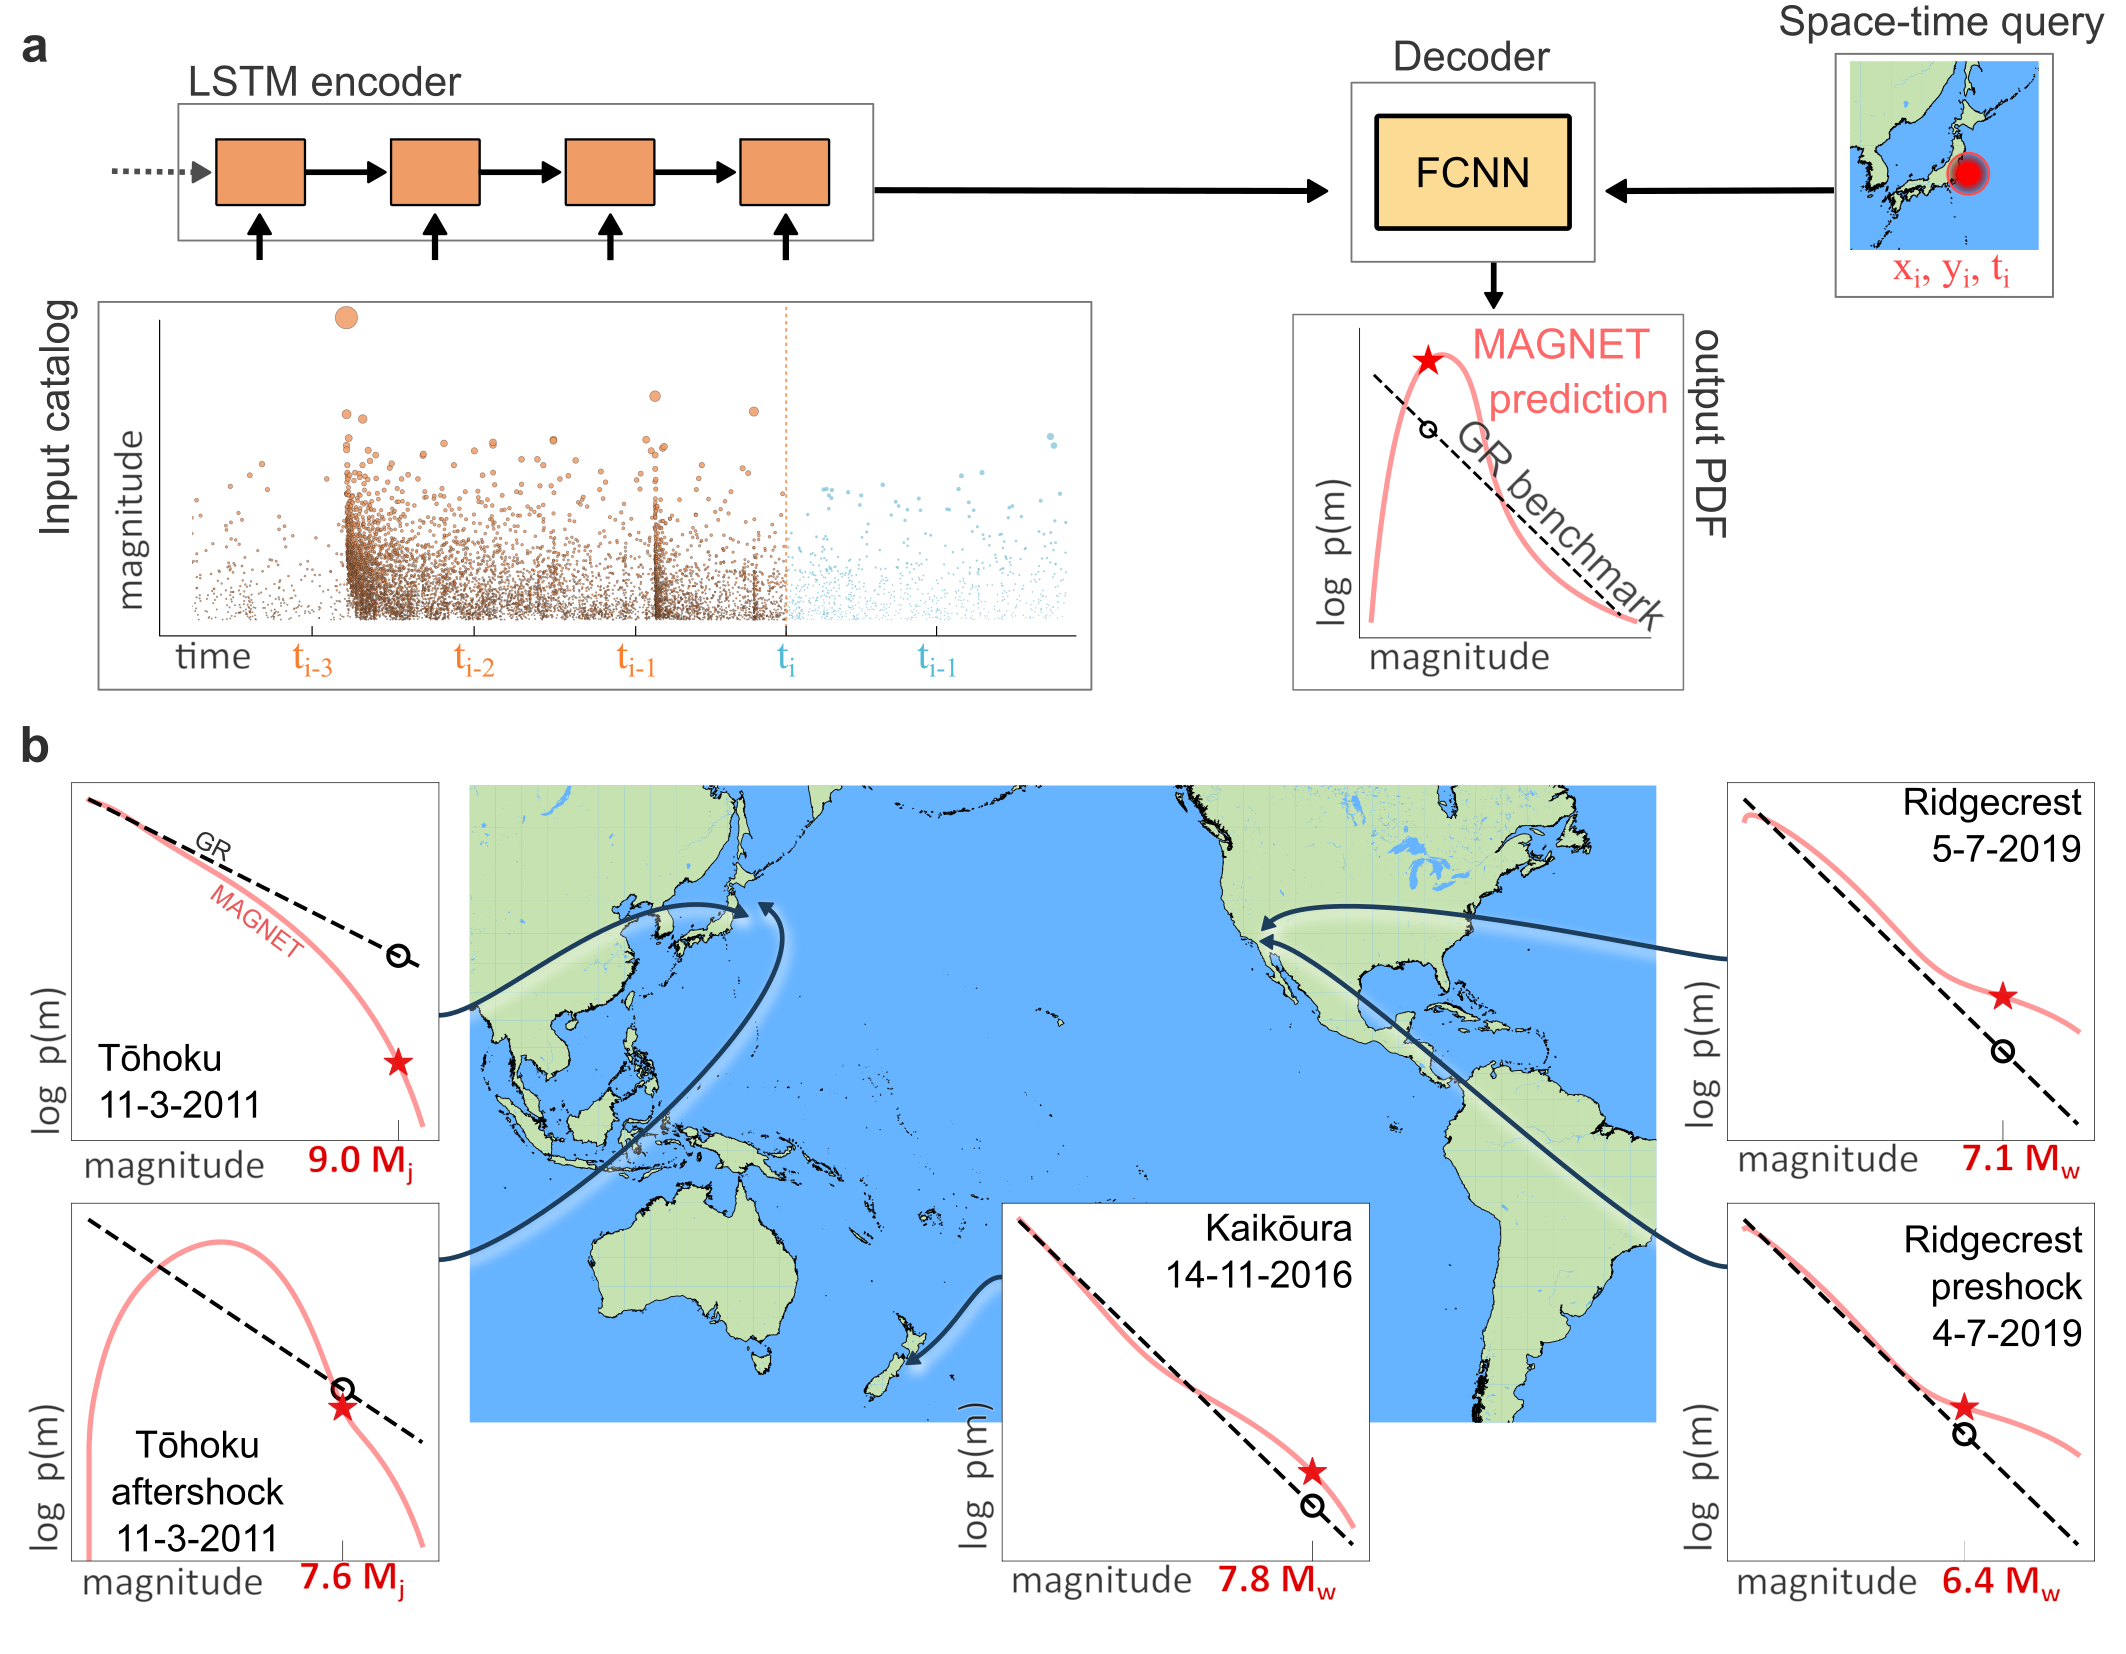
\includegraphics[width=1\textwidth]{figures/intro_fig.png}
	\caption{\textbf{a} MAGnitude Neural EsTimation model (MAGNET) task and architecture. Seismic history is continuously encoded using a Long Short-Term Memory neural network. For each earthquake, the encoded history up to its occurrence time ($t_i$) is concatenated with the time and location of the earthquake (``spacetime query''). The combined information is fed into a fully-connected neural network that outputs a probability density function (PDF) of the predicted magnitude at that time and location. \textbf{b} Performance on Major Earthquakes: MAGNET's resulting PDFs for a selection of well-known major earthquakes worldwide. The red curve represents the model's predicted PDF and the dashed black curve represents the Gutenberg-Richter (GR) magnitude-frequency distribution, a common naive benchmark. For most earthquakes shown here, the likelihood of the observed magnitude (red star) is higher for MAGNET than for the GR benchmark (black circle). Notably, the Tōhoku aftershock shows a qualitatively different behavior.
    }
\label{fig:intro_fig}
\end{figure}

All metrics reported in this work were evaluated over a time span that is not included in training period. The presented metrics demonstrate that our model consistently and significantly outperforms all benchmarks across all test regions, indicating a significant information gain in forecasting earthquake magnitudes prior to their occurrence.
%This finding directly suggests that the seismic system undergoes preparatory processes tailored to the impending event's magnitude before its initiation. Examining these results across multiple catalogs and regions highlights the robustness of our methodology and the generalizability of our conclusion, paving the way for further exploration of earthquake predictability.



\section{Results} \label{sec:results}
As explained above, the model outputs a PDF $p_{\textbf{x}_i, t_i}(m_i)$ for each earthquake in the test set. We denote by $\ell_i$ the log-likelihood of the observed magnitude $m_i$ as predicted by MAGNET, 
\begin{align}
    \mathcal{L} &= -\langle \ell_i \rangle\ , 
    &
    \ell_i&=\log\left(p_{\textbf{x}_i, t_i}(m_i)\right)
    \label{eq:likelihood}
\end{align}
 $\mathcal{L}$ is the average minus log-likelihood, which the model is trained to minimize.  The values of $\ell_i$ for MAGNET and the leading benchmark are presented in Extended Material Fig. \ref{fig:labels_likelihood}.
 

Figure \ref{fig:model_output}a shows the predicted PDFs for 100 randomly sampled events from the Southern California test set. The PDFs exhibit a clear trend: those that were calculated for higher-magnitude events are skewed towards larger magnitudes (warmer colors) compared to lower-magnitude events (cooler colors). This aligns with the expected behavior for an earthquake magnitude predictor. For comparison, the stationary GR distribution, the naive predictor which is independent of (recent) seismic history, is presented along the model's results.

This is a qualitative demonstration that the model works as expected. For a quantitative comparison, we calculate the $\mathcal{L}=-\langle \ell_i \rangle$ over all events in the test set, and benchmark it against state-of-the-art models:
the stationary Gutenberg-Richter (GR) distribution (fitted over the training set), and a few variants of a moving window GR approach~\cite{gulia_real-time_2019}. It is seen that MAGNET significantly and consistently outperforms all benchmarks across all three regions, as shown in Fig. \ref{fig:metrics}a-c. Further comparison to other benchmarks is given in Table \ref{tab:mean_ll_benchmarks_main_text}.

In addition to comparing the log-likelihood of the observed data, one can convert the prediction problem to a binary question: will the earthquake at the spacetime query $\textbf{x}_i, t_i$ have a higher magnitude than a threshold $m_t$? This can be easily calculated from the prediction, as the probability that $m_i>m_t$ is simply $\int_{m_t}^{\infty}p(m')dm'$.
This task, asking whether a given event will be a large earthquake, is more interpretable and can be evaluated using standard binary classification metrics such as area under receiver operator (ROC) curve \cite{Murphy} and under the interpolated precision-recall (PR) curve \cite{buttcher_information_2010} which suit better an imbalanced data set such as ours. Fig.~\ref{fig:metrics}d-f and g-i show these metrics for all three regions in examined and compare against the GR-variant models. Again, MAGNET outperforms all benchmarks.

Finally, Figure~\ref{fig:model_output}b presents the marginal probability density function (PDF) of magnitudes for MAGNET's prediction, $P(m)=N^{-1}\sum_i p_{\textbf{x}_i, t_i}(m)$. This represents the average probability distribution of magnitudes over the whole test set. It is seen that although the model was not constrained to do so, the average distribution aligns well with the ``uninformed'' GR distribution. That is, although MAGNET's prediction for each individual earthquake may deviate significantly from the GR distribution, it does reproduce this well known long-time behavior on average. It is also seen that the average prediction of the 300-event moving window GR deviates significantly from the GR distribution. We also observe that MAGNET's average prediction aligns well with the \emph{test set} GR distribution, rather than the training set, suggesting its ability to generalize beyond the training data. This observation is noticeable even more so in the New Zealand and Japan data sets presented in Extended Data Fig. \ref{fig:model_output_em}.

\begin{figure}[h!]
    \centering
    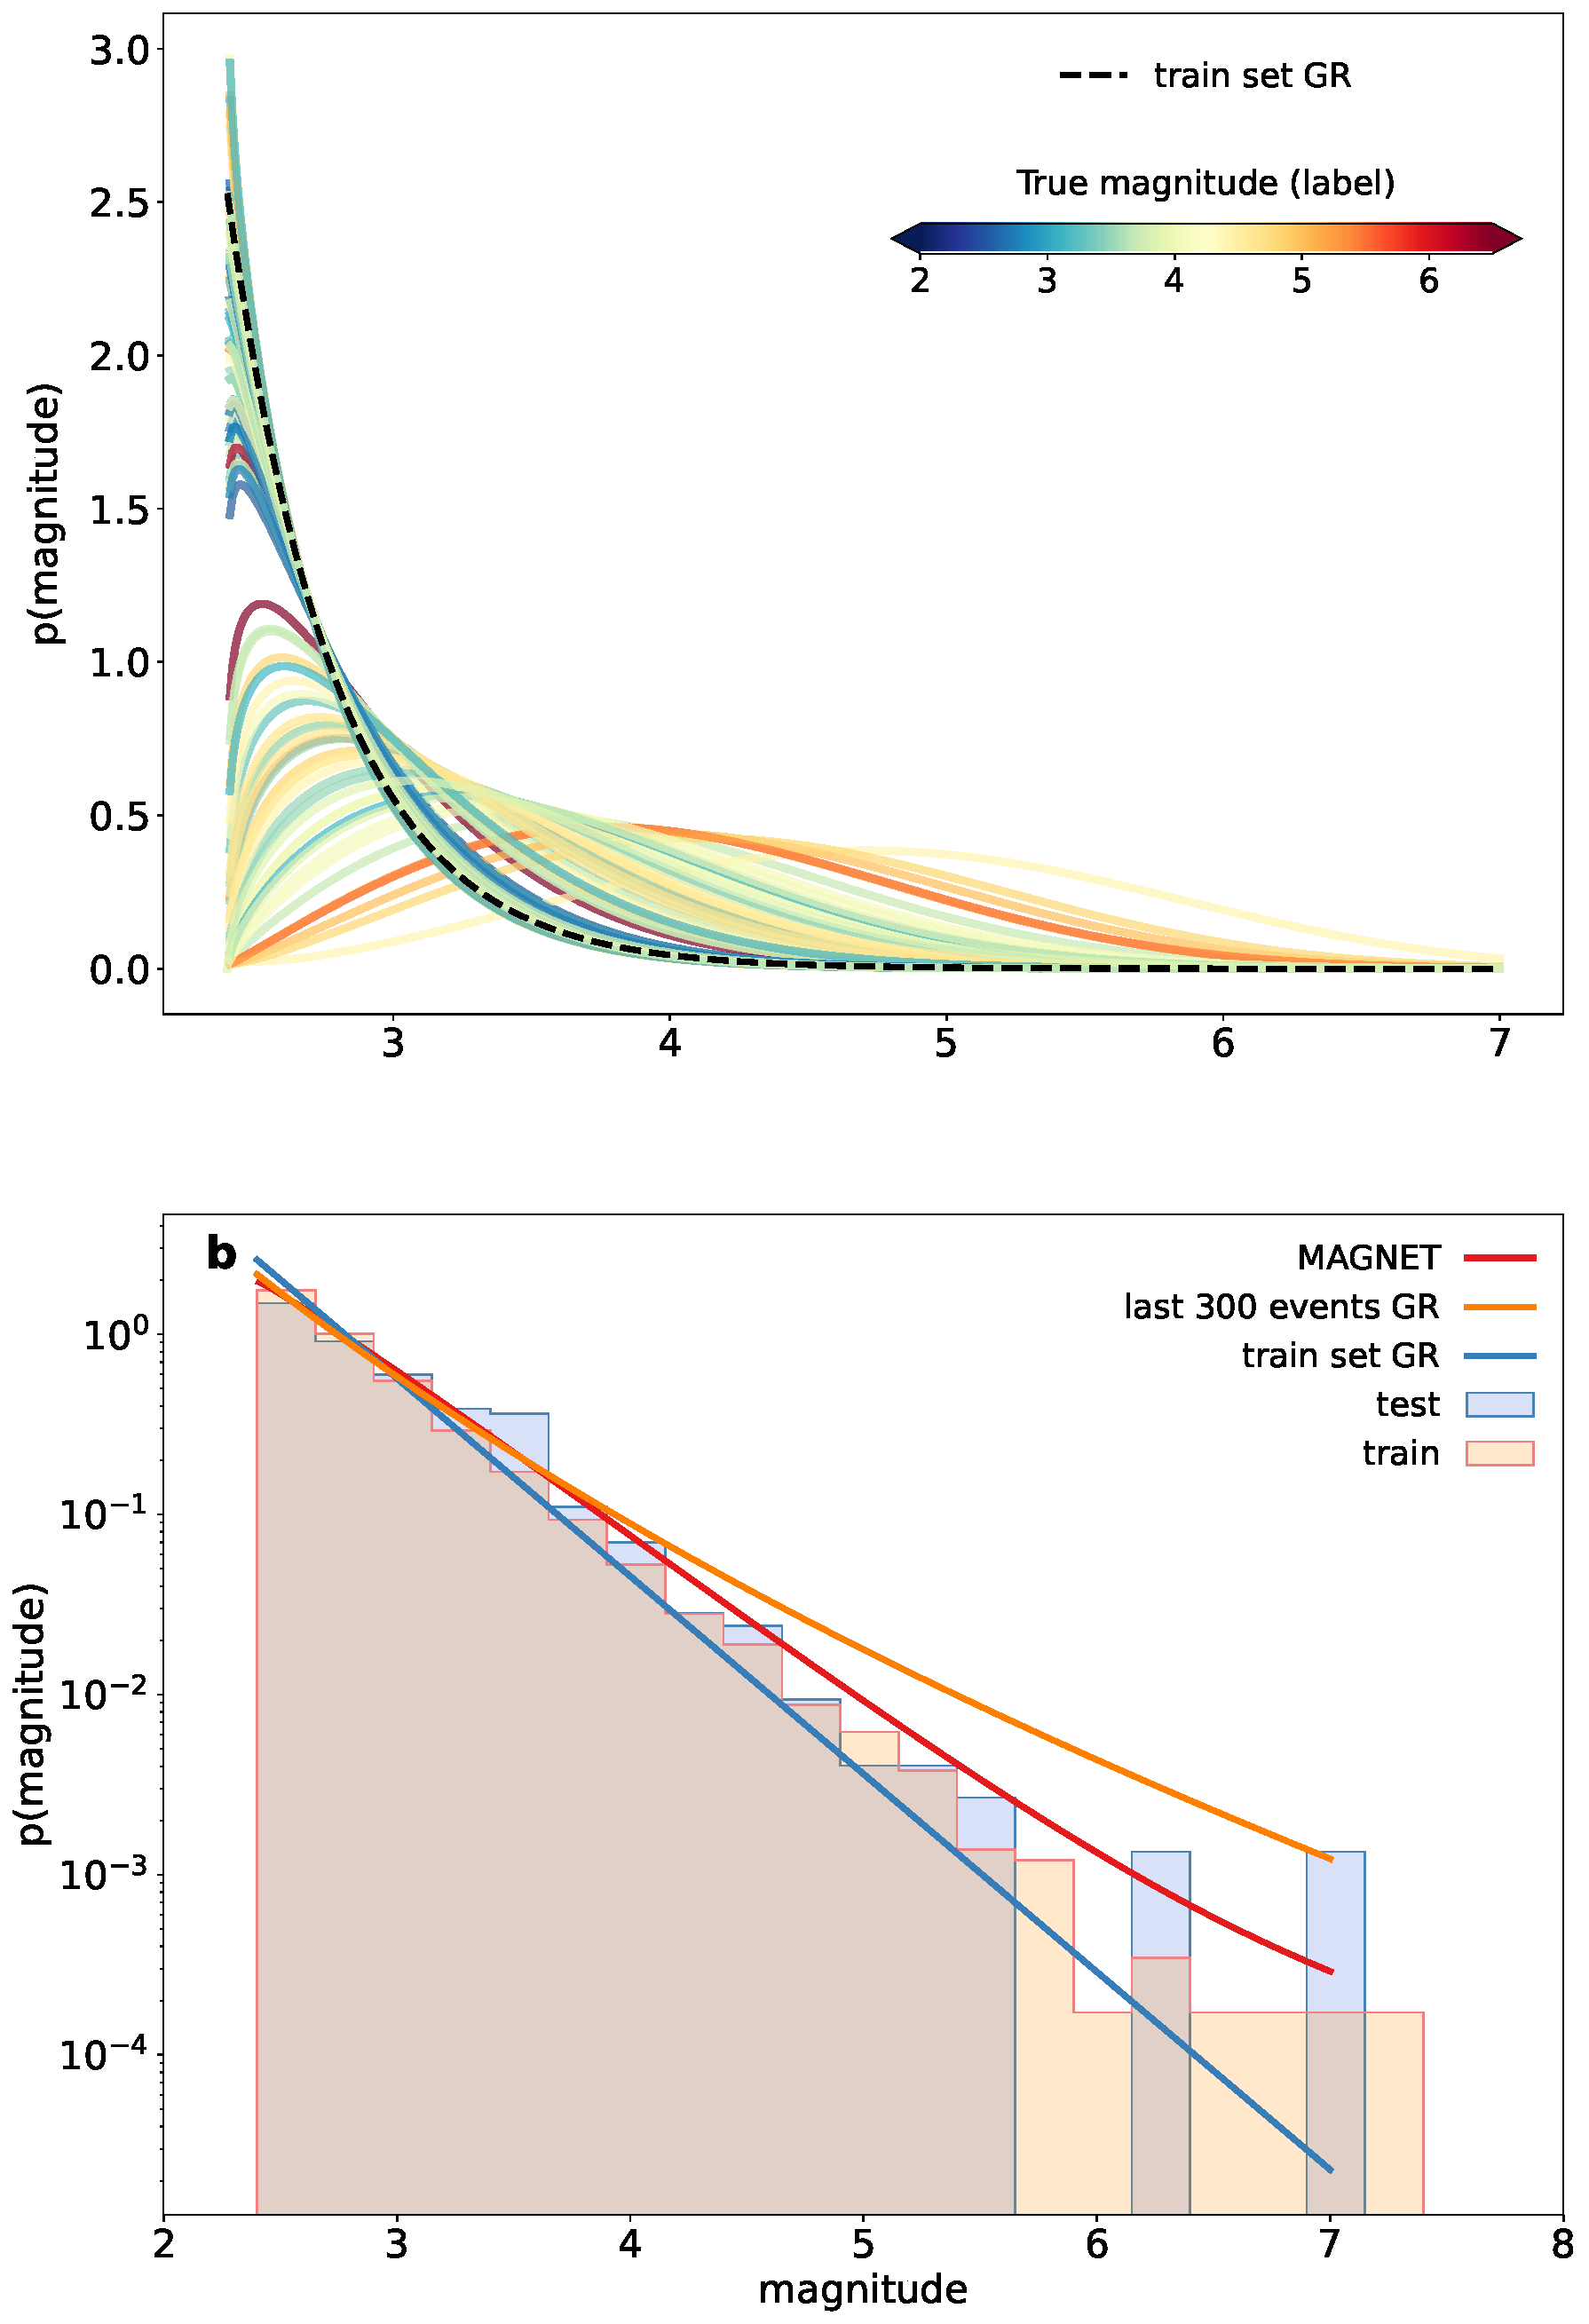
\includegraphics[width=0.5\textwidth]{figures/raw_results.pdf}
    \caption{
        \textbf{MAGNET's output}. \textbf{a}, Predicted magnitude PDFs produced by MAGNET for 100 randomly sampled events from the test set in the Southern California region. Curves are colored according to the magnitude of each earthquake event. It is seen that the PDFs for high magnitude events are generally skewed towards higher magnitudes, as expected from a predictive model. We superimpose the train set Gutenberg-Richter distribution (dashed black line).  \textbf{b}, Marginal magnitude distribution produced by MAGNET. That is, the average of all PDFs from the test set. It is seen that the marginal distribution closely resembles the GR distribution, though follows the test set distribution more precisely. In addition, we plot a similar marginal PDF for common benchmarks for the entire test set. Histograms of the train (and test) set are presented in orange (blue).
    }
    \label{fig:model_output}
\end{figure}

\begin{figure}[h!]
    \centering
    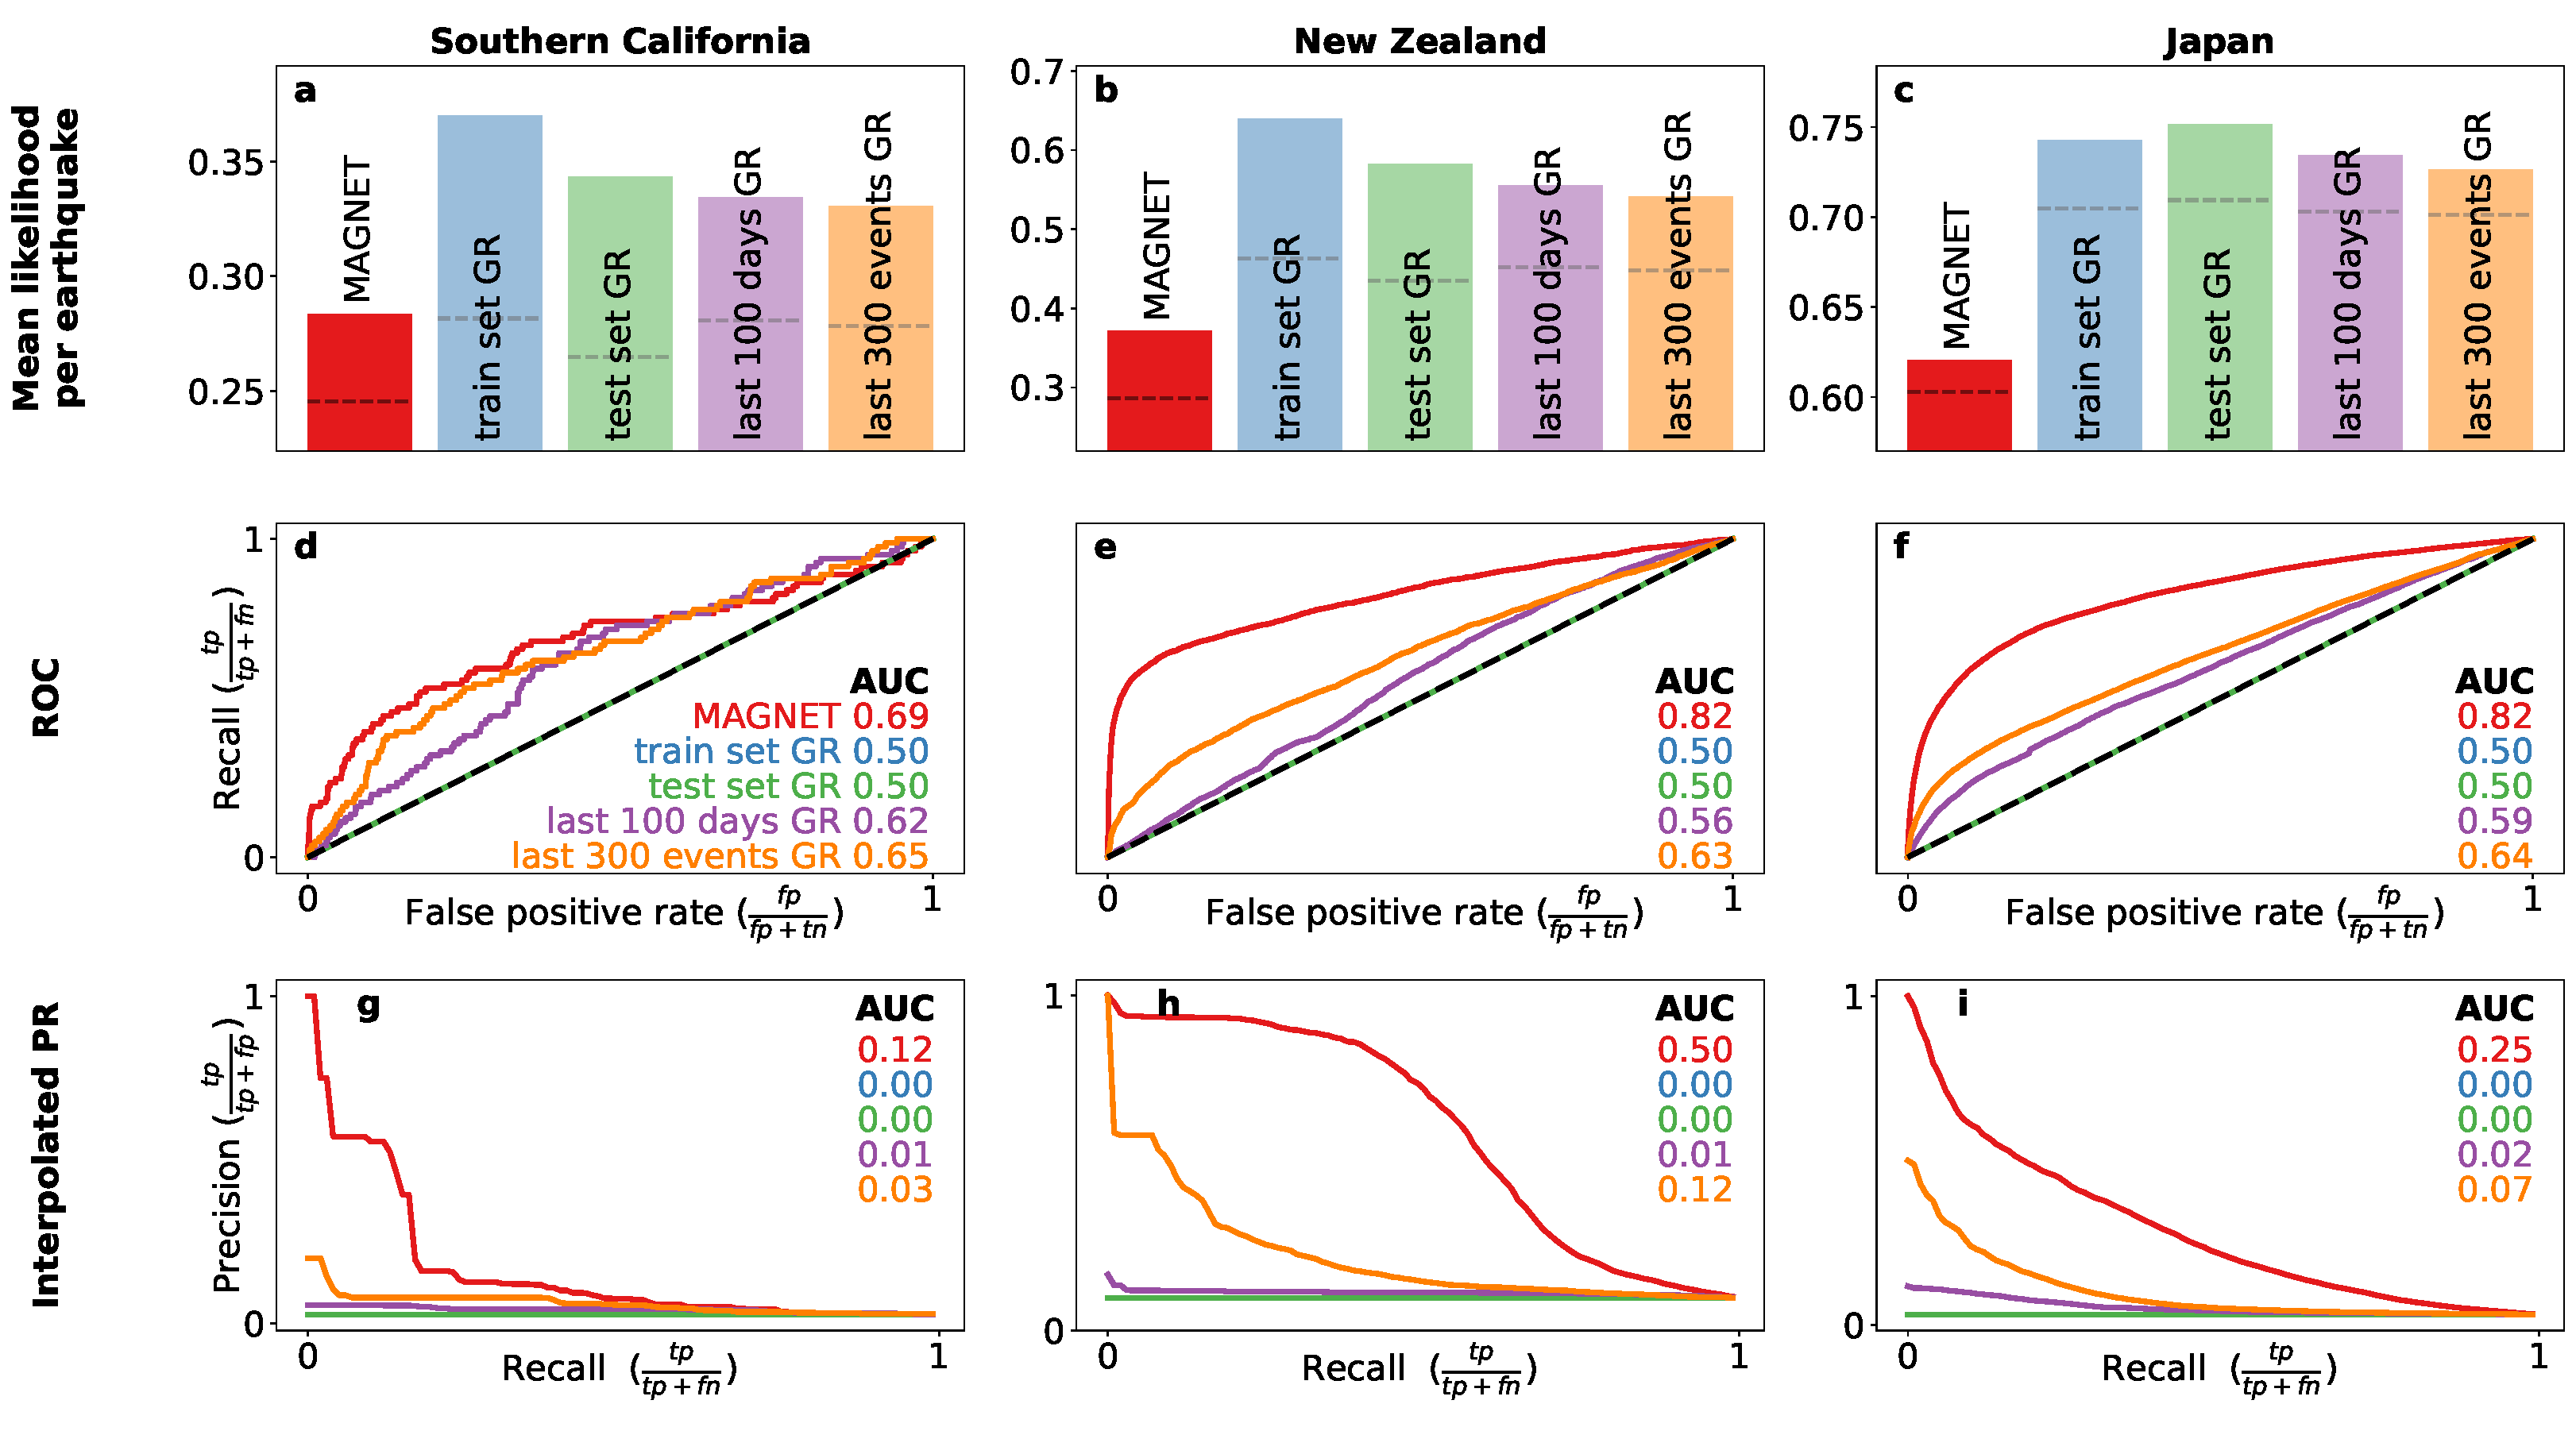
\includegraphics[width=1\textwidth]{figures/combined_barplots.pdf}
    \caption{
        \textbf{Benchmarking MAGNET. a}, \textbf{b}, \textbf{c}, Minus mean information content of our MAGNET model (red) and other common benchmark magnitude predictors (see labels on bars in the figure). A lower score indicates a better preforming model. Scores conditioned above the temporal incompleteness are marked by the horizontal dashed line on each corresponding bar. \textbf{d, e, f}, Receiver Operating Characteristic (ROC) and \textbf{g, h, i} the interpolated precision-recall (PR) curve for a binary classifier determining the existence of a large ($m>=4$) event. The performance of such a classifier can be quantified by the area under the curve (AUC), noted in each frame, color coded identically to the bar plots. For the AUC metrics, a higher score indicates a better preforming classifier.
        }
        \label{fig:metrics}
\end{figure}


\begin{table}[h!]
    \centering
    \includegraphics[width=1\textwidth]{figures/score_tables_main.pdf}
    \caption{Mean score, $\mathcal{L}$, for various tested benchmarks. $\mathcal{L}$ is computed by Eq. \ref{eq:likelihood}. Lower score indicates a better magnitude predictor, best score in column is indicated in bold. First 3 columns display scores for the raw calculation of $\mathcal{L}$, middle and right column triplets display the scores for the temporally and spatially conditioned $\mathcal{L}$ scores, respectively.
    }
    \label{tab:mean_ll_benchmarks_main_text}
\end{table}
   
    
\begin{figure}[h!]
    \centering
    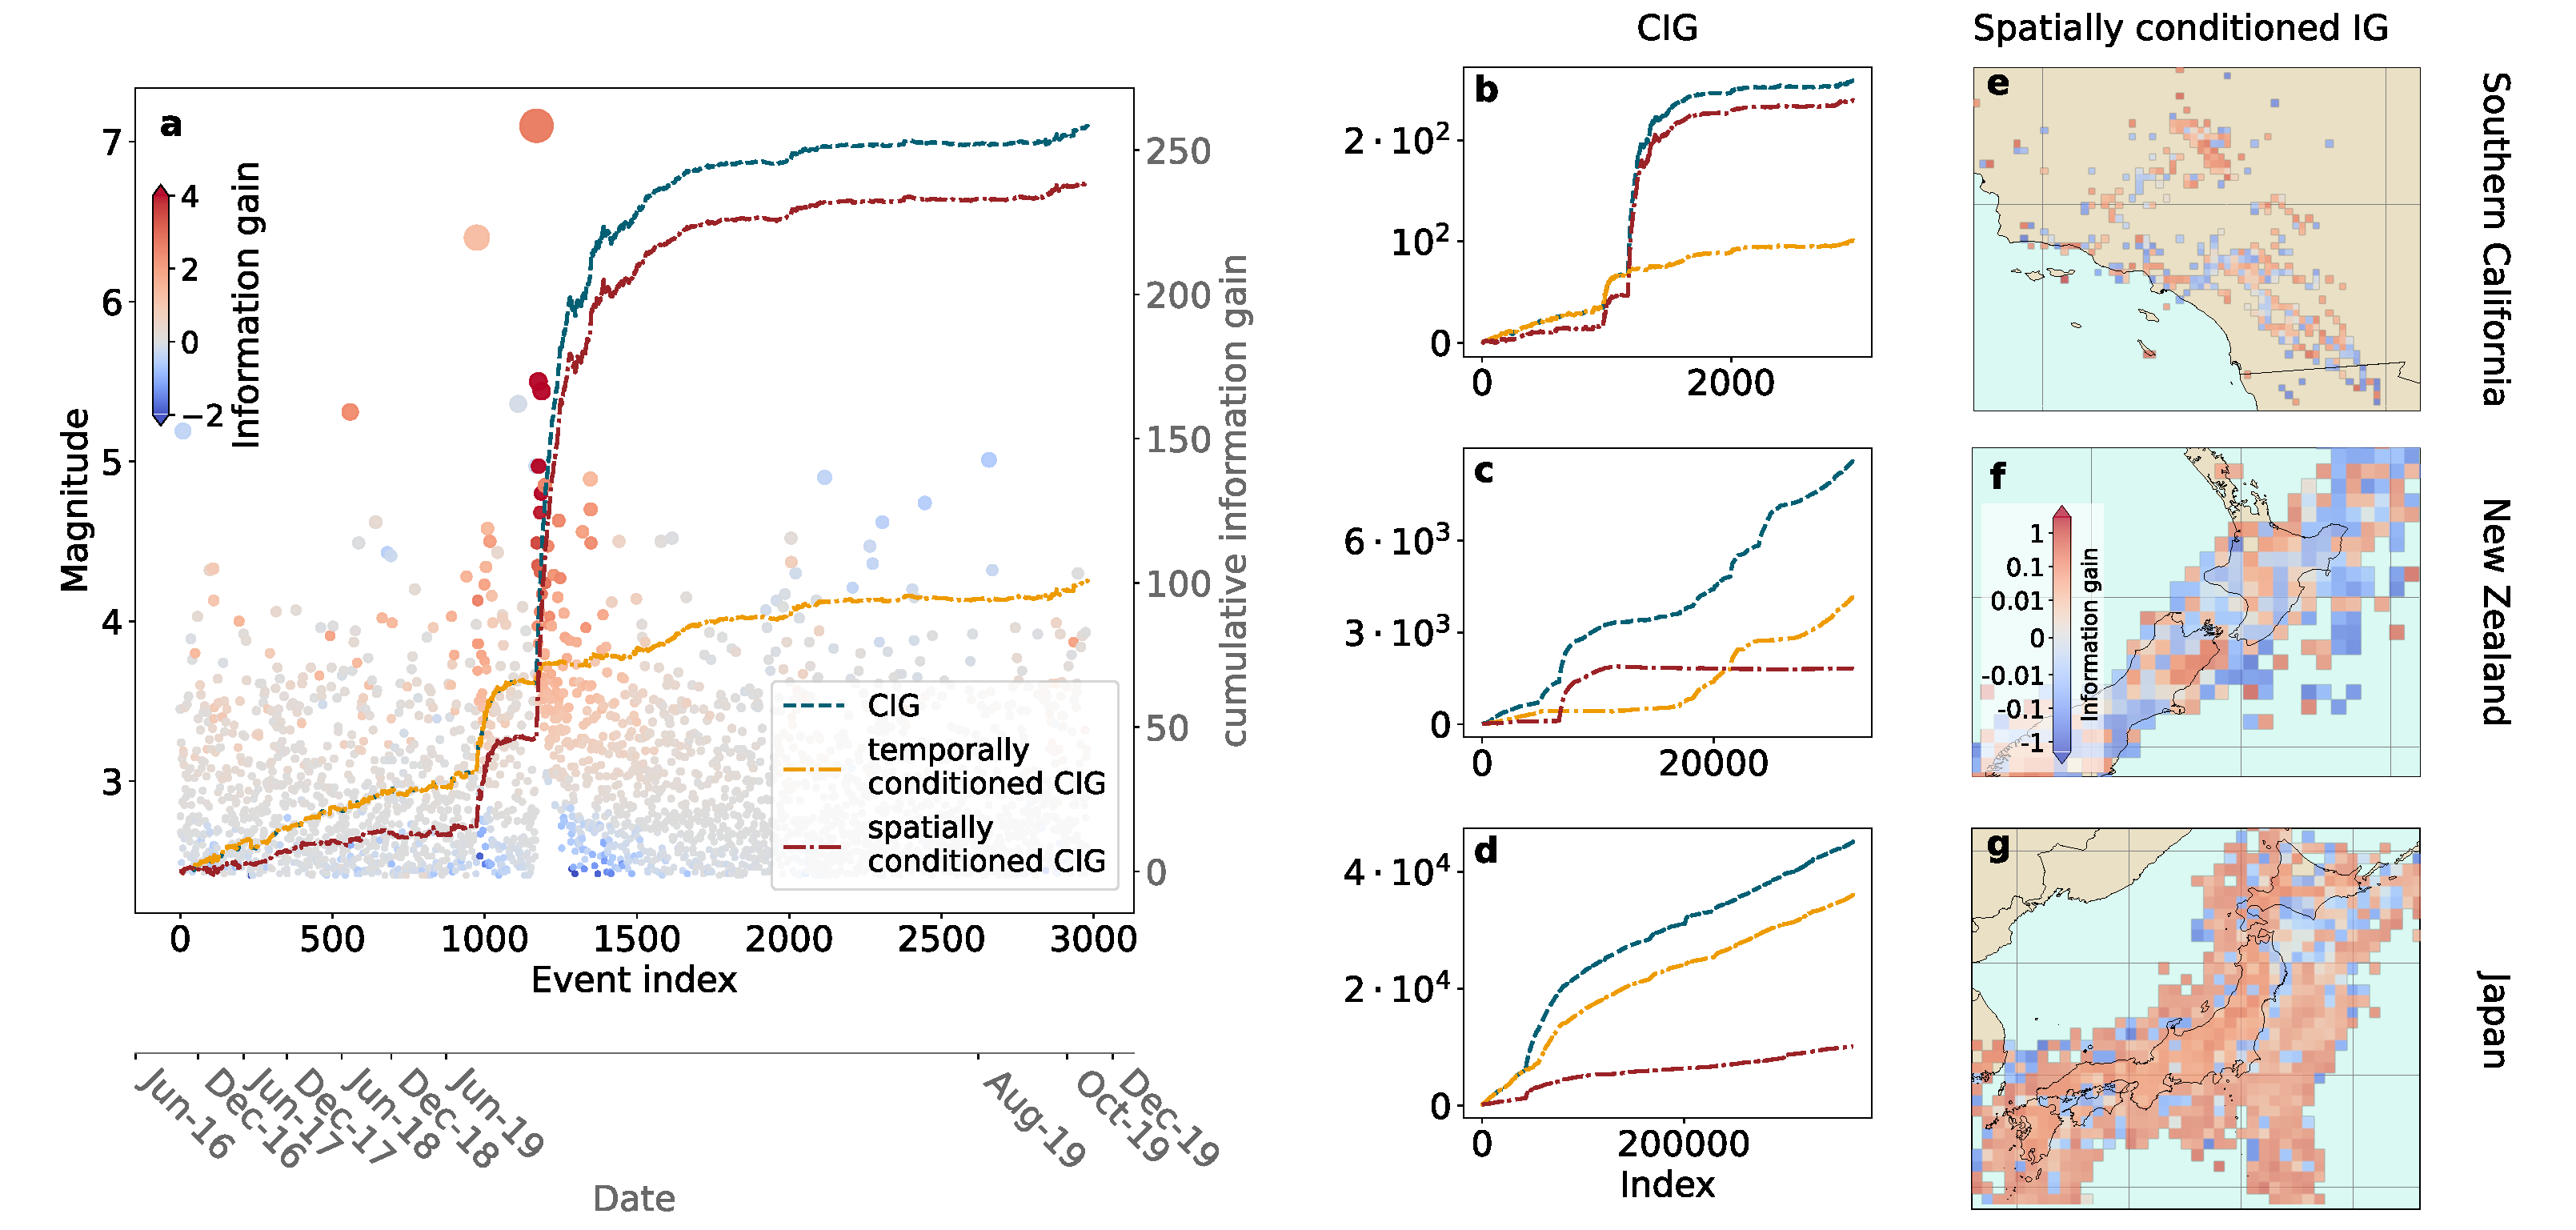
\includegraphics[width=1\textwidth]{figures/info_over_time_hauksson.pdf}
    \caption{
        \textbf{Information gain in MAGNET. a}, Information gain of individual events in the Southern California test set. Scattered dots indicate magnitude at event index, colored by the information gain per event (scale indicated by colorbar), here warm is an advantage for MAGNET, while cool is an advantage for the benchmark. Secondary horizontal axis (grey) indicates corresponds origin time. Cumulative Information gain (CIG) (dashed blue), temporally conditioned CIG (dashed yellow) and spatially conditioned CIG (dashed red) curves are superimposed on the scatter, demonstrating a constantly increasing function. \textbf{b-d}, Information gain (dashed blue) temporally conditioned CIG (dashed yellow) and spatially conditioned CIG (dashed red) curves for Southern California, New Zealand and Japan test sets, respectively, all three regions examined in this study. An exception from the increasing trend can be observed for the spatially conditioned CIG of New Zealand (red curve in c). \textbf{e-g} Spatial distribution of spatially conditioned information gain for all regions in study. Maps show the difference in mean information content per bin, model's advantage is indicated by warm colors, disadvantage by cool colors, as defined by the colorbar adjacent to f.
    }
    \label{fig:info_gain_over_time}
\end{figure}
    

It is interesting to examine MAGNET's information gain per event, which is quantified by the difference in log-likelihood (LL) of the observed magnitude, 
\begin{equation}
    \Delta \ell_i = \log{p_{\pmb{x_i}, t_i}^{(MAGNET)}(m_i)} - \log{p^{(GR)}(m_i)}
    \label{eq:information_gain}
\end{equation}
%This equation measures the amount of information gained by using our MAGNET model rather than the GR benchmark, for a specific event. 
Analyzing this quantity per event across the entire test set reveals patterns indicating where and when our model achieves its advantage. Fig. \ref{fig:info_gain_over_time}a shows the test set for Southern California events magnitudes by their running index, colored according to the information gain as defined in Eq. \ref{eq:information_gain}. This time-domain representation allows us to track the cumulative information gain, calculated over the entire test set and displayed as the blue dashed line in the figure.
The predominantly increasing trend in cumulative information gain suggests that our model is consistently advantageous as opposed to identifying some local trends such as immediate aftershock sequences. Notably, for the Southern California data set, the most rapid information gain occurs during the aftershocks of the two Ridgecrest earthquakes. Surprisingly, even the pre-shock and main shock events demonstrate positive information gains over the GR benchmark, with $\Delta \ell$ values of $0.5$ and $1.4$ nats (log(2) nat = 1 bit), respectively.

Our analysis reveals a persistent increase in information gain across the test set for all investigated regions (Fig. \ref{fig:info_gain_over_time}b-d). Specifically, we show an average information gain of $>0.1$ nats per earthquake in the same region in Japan where Ogata et.~al.~\cite{ogata_exploring_2018} found no information gain. Similar plots for the other studied regions are shown in Extended Material Fig.~\ref{fig:nz_japan_info_gain}.

\section{Interpretation and caveats}
At this point, it is clear that MAGNET is able to extract information about the magnitude of specific earthquakes, prior to their occurrence. However, such an information gain may potentially result not from the fact that the underlying physical process is predictable (at least to some extent), but from various measurement and modeling artifacts. 

An obvious such artifact is ``short-time incompleteness'' (STI): the fact that immediately following a large event the signal of subsequent small events might be buried in the coda of the mainshock~\cite{kagan_short-term_2004, stockman_forecasting_2023}. Thus, immediately after a large event it is less likely that a small event will be included in the catalog, not because it did not occur, but rather because it was not detected. Indeed, our model consistently allocates less probability mass to low magnitudes shortly after large events (see the Tohoku aftershock in Fig.~\ref{fig:intro_fig}b), and some of the information gain may be attributed to this effect.  

In order to factor the effect of STI from the information gain calculation, we recalculate the likelihood score of each event, $p(m_i)$, conditioned on the magnitude exceeding a threshold, $\Tilde{m}$, which is the time-dependent completeness magnitude:

\begin{equation}
    p \left( m \vert m_i > \Tilde{m} \right) = \frac{p_{\pmb{x}_i, t_i}(m)} {\int_{\Tilde{m}}^{\infty} p(m') dm'}
    \label{eq:conditioned_likelihood}
\end{equation}

The instantaneous completeness magnitude, $m_c(t)$, is defined as the minimal magnitude above which all earhtquakes can be detected. If we choose $\tilde m \geq m_c$ then, by definition, the model cannot present an information gain due to the STI effect.

We thus take $\Tilde{m}=m_c(t)$, which we estimate dynamically using the maximum curvature method \cite{wiemer_minimum_2000} within a window of 150 past and 150 current and future events. The resulting $m_c(t)$ curves are presented in the Extended Material Fig. \ref{fig:temp_incompleteness}. The conditioned cumulative information gain (CIG) is then recalculated and presented as the yellow dashed curved in Fig.  \ref{fig:info_gain_over_time} for all three tested regions. 
Indeed, factoring out the temporal incompleteness reduces the information gain, though it is still significant: evidently, the conditioned CIG curves show a steadily increasing trend. the horizontal dashed lines on the bars in Fig \ref{fig:metrics}a-c indicate the mean conditioned scores, also presented in Table \ref{tab:mean_ll_all_benchmarks}. EM Table \ref{tab:mean_ll_benchmarks_main_text} displays the conditioned scores for all benchmarks tested in this study.

Similarly to the temporal domain, a spurious information gain may also be caused by temporally constant but spatially varying properties. For example, fault stresses, geometry and lithology may change in space resulting in spatially-dependent GR distribution \cite{amitrano_brittle-ductile_2003, scholz_stress_2015, herrmann_revealing_2022, taroni_earthquake_2023}, and the local completeness magnitudes is also generally spatially dependent. In such a case, the information gain of MAGNET does not imply that the magnitudes are correlated in time. 
To examine this, we preform two additional tests. First, we construct a spatially dependent GR distributions where $m_c$ is held constant ($=m_c^{\mbox{\footnotesize (train set)}}$). MAGNET outperforms the spatially varying GR benchmark for all regions in the unconditioned $\mathcal{L}$ score, as can be seen in EM Table \ref{tab:mean_ll_all_benchmarks}. The spatially varying GR shows an advantage over MAGNET for solely the New Zealand data set for the temporally conditioned $\mathcal{L}$. This advantage may arise from a the measurement artifact of spatial variation of $m_c$ originating from the properties of the seismic network.

In order to account for such spatially dependent artifacts we preform a simialrecond calculation. We once again condition MAGNET's results on a threshold according to Eq. \ref{eq:conditioned_likelihood}, this time choosing a spatially varying completeness $\Tilde{m}=m_c(x,y)$. We estimate $m_c(x,y)$ for a grid of coordinates spaced every $0.1^\circ$, for all events within a square centered at each grid point, with a side length of $0.2^\circ$. 

The spatially conditioned CIG curves are shown as the red dashed curve in Fig. \ref{fig:info_gain_over_time} for all three regions. It is a steadily increasing function for the Southern California and Japan data sets. In the New Zealand data set the curve shows an initial increase followed by a plateau after the first sequence of major events (the 2016 Te Araroa and Kaikōura earthquakes). This may indicate that a good portion of this information gain followed by these earthquakes originate in the spatial incompleteness artifact. Nevertheless, the overall score still shows an advantage for our model over the test set. Fig. \ref{fig:info_gain_over_time}e-g show the spatial distribution of MAGNET's advantage over the GR benchmark. All three regions exhibit a spatially diffuse pattern, suggesting that information is not gained solely from any one specific area.


\section{Implications and Outlook}
In this work we have used neural based models to find statistical dependencies between earthquake magnitudes and seismic history. Since our model is provided with the known location and timing of an event and is only tasked with predicting its magnitude, we have separated out the question of rate and location of earthquakes, and directly probe whether their magnitude is history dependent. MAGNET shows robust and significant information gain, even after accounting for possible measurement artifacts such as temporal or spatially dependent incompleteness, compared against a host of benchmarks. Our results indicate that some information about the magnitude of a specific event can be extracted, on average, from the regional seismic history in the form of a simple hypo-center catalog. 

%A corollary follows this finding: for some earthquakes, the magnitude might be partially predetermined before the earthquake is initiated. 

If true, this means that the seismic patterns preceding large events are distinguishable, at least to some extent, from those preceding ``background'' activity. A similar claim was recently raised by Ben~-~Zion and Zaliapin\cite{ben-zion_localization_2020}, which show trends in statistical properties of the seismicity prior to fault-size events, though a direct linkage between the two observation requires further investigation. 

In the future, it will also be interesting to examine MAGNET's prediction on query coordinates in the vicinity (either in space or time) of true events, producing a space-time hazard map, which may be used to inform existing forecasting and early-warning systems. This can also be done by constructing a different model, trained to estimate the magnitude of an upcoming earthquake ahead of the origin time, examining how it depends on the lead time and distance from the event location. 
It would also be interesting to understand what are the statistical features of seismicity that our model identifies, which may be done using various explainability analyses~\cite{sturmfels_visualizing_2020, zhang_survey_2021, liu_interpretable_2023}. Potentially, ablation tests \cite{meyes_ablation_2019, sturmfels_visualizing_2020} can be applied to extract heuristic, more simplified dependencies between statistical trends in the seismic history to trends in the resulting PDF.


\section{Possible affects on operational earthquake forecasting and prediction}
Identifying precursory patterns in the seismic history can advance the effort of earthquake prediction a great deal\cite{mousavi_deep-learning_2022, mousavi_machine_2023, mignan_neural_2020, karimpouli_explainable_2023, bergen_machine_2019}. Nevertheless, discovering such signals with enough accuracy to prove useful for operational systems may still be further down the road.
However, an immediate application of the model may be a quick estimation of magnitude for early warning systems. Such a system does not require additional data sources or assumptions on the model as the timing and location of the earthquake to be estimated are known or estimated. 
Another immediate application is to incorporate such a history-dependent magnitude distribution into point-process rate forecasting models, such as the epidemic type aftershock sequence model (ETAS) or similar \cite{ogata_statistical_1988, ogata_statistics_2017, dascher-cousineau_using_2023}. As discussed above, such models currently assume no statistical dependence of the magnitude. Since larger earthquakes produce more aftershock, a more accurate estimation of magnitudes will have a positive compounding effect on the resulting statistics.

% \neri{I bet the reviewer will want us to talk about limitations and improvements to the model but maybe we can wait and see}


% There are two bibliographies in Nature papers. One for the main text, and one for the Methods and Extended Data sections. The numbering is sequential, meaning that the reference section for the Methods and Extended Data section starts after the last number from the main reference section. References should not appear in both sections. Any reference used in Methods or Extended Data that also appears in the main bibliography should *only* appear in the main bibliography.
\let\oldbibliography\thebibliography
\renewcommand{\thebibliography}[1]{%
  \oldbibliography{#1}%
  \setlength{\itemsep}{10pt}%
}
% \bibliography{bibliography}
% \bibliography{bib-article.bib}
\newpage
\bibliography{Magnitude_prediction_paper}

\let\oldthebibliography=\thebibliography
\let\oldendthebibliography=\endthebibliography
\renewenvironment{thebibliography}[1]{
    \oldthebibliography{#1}
    % The number here (34 is an example) is the number of references in the main bibliography, and thus defines the starting number of the first reference in the Methods and Extended Data bibliography.
    \setcounter{enumiv}{62}
}{\oldendthebibliography}

% Figure legends appear after the text, not placed in the text. Do not include the actual image files in the article. Images are submitted as separate files. During the first submission to the journal, you can include the images in the article file for readability, but if you pass the reviews, they will want the images removed from the main article.
\newpage
\unnumbered

\unnumbered
\section{Methods}
\subsection{Neural architecture}
A detailed visual of the model's architecture is presented in Extended Data Fig. \ref{fig:architecture}. The catalog is used as an input into three distinct encoding components:
\subparagraph{\textbf{Recent Earthquakes Encoder}} Calculates a set of predefined (non trainable) functions on various past time windows. The result is then used as input to a LSTM NN. A detailed description of this encoder is given in Zlydenko et.~al.~\cite{zlydenko_neural_2023}. 

\subparagraph{\textbf{Seismicity Rate Encoder}} Computes a rough estimation of the amount of energy released in a given region around the query coordinate, in a given past time window. The result is then input to a LSTM NN. A detailed description of this encoder is found in Zlydenko et.~al.~\cite{zlydenko_neural_2023}.

\subparagraph{\textbf{Spacetime Query Encoder}} Time is represented as the time difference from the most recent past event, in seconds. No further processing is done in this encoder.

Outputs of all encoders are concatenated and fed to a Fully Connected Neural Network (FCNN). The sizes of layers in the FCNN, as the number of layers themselves, are optimized by cross validation. A $tanh$ activation is used for the hidden layers, and a $\texttt{softplus}$ as an activation on the output layer. 

\subsection{Loss metric}
To obtain the Probability Density Function (PDF) of the magnitudes ($p(m)$) for each query coordinates ($\textbf{x}_i, t_i$) we maximize the likelihood, $\mathcal{L} = -\langle \ell_i \rangle$, where $\langle \cdot\rangle$ is the mean over all examples in the set. The PDF is taken to be a mixture of two stretched and shifted Kumaraswamy distributions~\cite{kumaraswamy_generalized_1980}:
\begin{equation}
    p\left( m \right)
    \equiv
    \sum_{j=1,2} \frac{A_j}{\sigma}a_jb_j\left(\frac{m-m_c}{\sigma}\right)^{\left(a_j-1\right)}\left(1-\left(\frac{m-m_c}{\sigma}\right)^{a_j}\right)^{\left(b_j-1\right)}
\end{equation}
Here $a_j, \ b_j$ are the parameters of the Kumaraswamy distribution. $m_c$ is the train set's completeness magnitude. $m_c$ together with $\sigma$ define the support of $p(m)$ to $[m_c, m_c+\sigma]$. $A_j$ is a normalization prefactor, with $j$ the summation index defining the PDF mixture.

\subsection{Definition of benchmark models}
\subparagraph{Last $n$ events} The Gutenberg- Richter (GR) distribution fitted for the past $n$ events. This method follows the method presented in Gulia \& Wiemer\cite{gulia_real-time_2019} for constructing a b-value time-series. If in the last $n$ events there are less than 10 earthquakes of magnitudes above $m_c^{train}$, then more events from the past are included, until this condition is met. $m_c^{train}$ is estimated using the maximal curvature method\cite{wiemer_minimum_2000}.

\subparagraph{Last $d$ days} The Gutenberg- Richter (GR) distribution fitted for the events in the past $d$ days. This method is identical to the previous method in all but the definition of the window selection.

\subparagraph{Spatially varying GR} Estimation of the local $b$ value is done by following the method of Taroni et.~al.~\cite{taroni_highdefinition_2021}. Seismicity data is 
binned into $0.1^\circ \times 0.1^\circ$ bins, and the GR distribution is fitted for each bin. $b$ for a specified location $x_i$ is calculated by the average of all $b$ values in bins within 30km around $x_i$. Estimations which consider less than 150 events are discarded.

\subparagraph{Kernel density estimation (KDE) of last n events} Selecting the last $n$ events (similar to described in \textit{last $n$ events}) we copmute the KDE estimation of the magnitude PDF, using the 'scott' estimator bandwidth\cite{scott_2015}. This is implemented using the SciPy tool\cite{scipy_2020}. The resulting PDF is used as the prediction of the magnitude.

\subsection{Measurement of incompleteness}
\subparagraph{Temporal incompleteness} Temporal incompleteness is measured at the times of events by fitting the completeness magnitude to a window of 300 events: 150 past events, 1 current event, 149 future events. The window is constructed by the same algorithm as in the \textit{Last $n$ events benchmark}.

\subparagraph{Spatial incompleteness} Spatial incompleteness is calculated for a grid of coordinates, spaced by $\theta^\circ$ degrees, covering the relevant region. $\theta$ is set to 0.1 for Southern California and 0.5 for New Zealand and Japan data sets. Calculation is done using train set's events. The value per point is calculated using the maximal curvature method\cite{wiemer_minimum_2000}, over the nearest, at least 100 events, with a minimal radius of $\theta^\circ$. In cases where the the nearest 100 events span over a radius of $2^\circ$ the data point is considered invalid. Events from the test set are divided into bins of $\theta^\circ$ centered around the point for which $m_c(x,y)$ was computed. Events are assigned with the $m_c$ value of their bin.


\section*{Data and code availability}
The datasets analysed during the current study are available in the relevant references mentioned throught the article.
The code for analysing the data is available in \textcolor{red}{\textbf{**link TBA**}}

Country borders in this work are plotted using data from https://geojson-maps.kyd.au/ .
% This is a required section. Guidelines for data availability: \url{https://www.nature.com/documents/nr-data-availability-statements-data-citations.pdf}.

\newpage
\renewcommand\refname{Methods References}
\begin{thebibliography}{10}
\bibitem{zlydenko_neural_2023}
Zlydenko, O. et al. A neural encoder for earthquake rate forecasting. Sci Rep 13, 12350 (2023).
\bibitem{taroni_highdefinition_2021}
Taroni, M., Zhuang, J. \& Marzocchi, W. High‐Definition Mapping of the Gutenberg–Richter b‐Value and Its Relevance: A Case Study in Italy. Seismological Research Letters 92, 3778–3784 (2021).
\bibitem{scott_2015}
Scott, David W. Multivariate density estimation: theory, practice, and visualization. John Wiley \& Sons, 2015.  
\bibitem{scipy_2020}
Virtanen, P., Gommers, R., Oliphant, T.E. et al. SciPy 1.0: fundamental algorithms for scientific computing in Python. Nat Methods 17, 261–272 (2020).





\end{thebibliography}


\newpage
\section*{Acknowledgements}
We thank Yehuda Ben-Zion, Assaf Inbal, Kelian Dascher-Cousineau, David Marsan and Eugenio Lippiello, Jiancang Zhuang and Yosihiko Ogata. for thoughtful discussions. YBS is supported by ISF grant 1907/22 and by Google Gift grant.

\section*{Author Contributions}
N.B., O.Z., O.G. and Y.B.S. designed the research. N.B. conducted the experiments. N.B., O.G. and Y.B.S. preformed the statistical analysis. N.B. and O.Z. wrote the code base. N.B. and Y.B.S. wrote the manuscript. All authors reviewed the manuscript.

\section*{Author Information}
The authors declare no competing interests. Please contact Yohai Bar-Sinai \href{mailto:ybarsinai@gmail.com}{ybarsinai@gmail.com} or Neri Berman \href{mailto:neriberman@gmail.com}{neriberman@gmail.com} for correspondence and requests, including questions regarding reprints and permissions.


\newpage
\begin{table}[h!]
    \centering
    \includegraphics[width=1\textwidth]{figures/score_tables_EM.pdf}
    \caption{Mean score, $\mathcal{L}$, for all tested benchmarks. $\mathcal{L}$ is computed by Eq. \ref{eq:likelihood}. Lower score indicates a better magnitude predictor, best score in column is indicated in bold. First 3 columns display scores for the raw calculation of $\mathcal{L}$, middle and right column triplets display the scores for the temporally and spatially conditioned $\mathcal{L}$ scores, respectively.
    }
    \label{tab:mean_ll_all_benchmarks}
\end{table}



\newpage
\begin{figure}[h!]
    \centering
    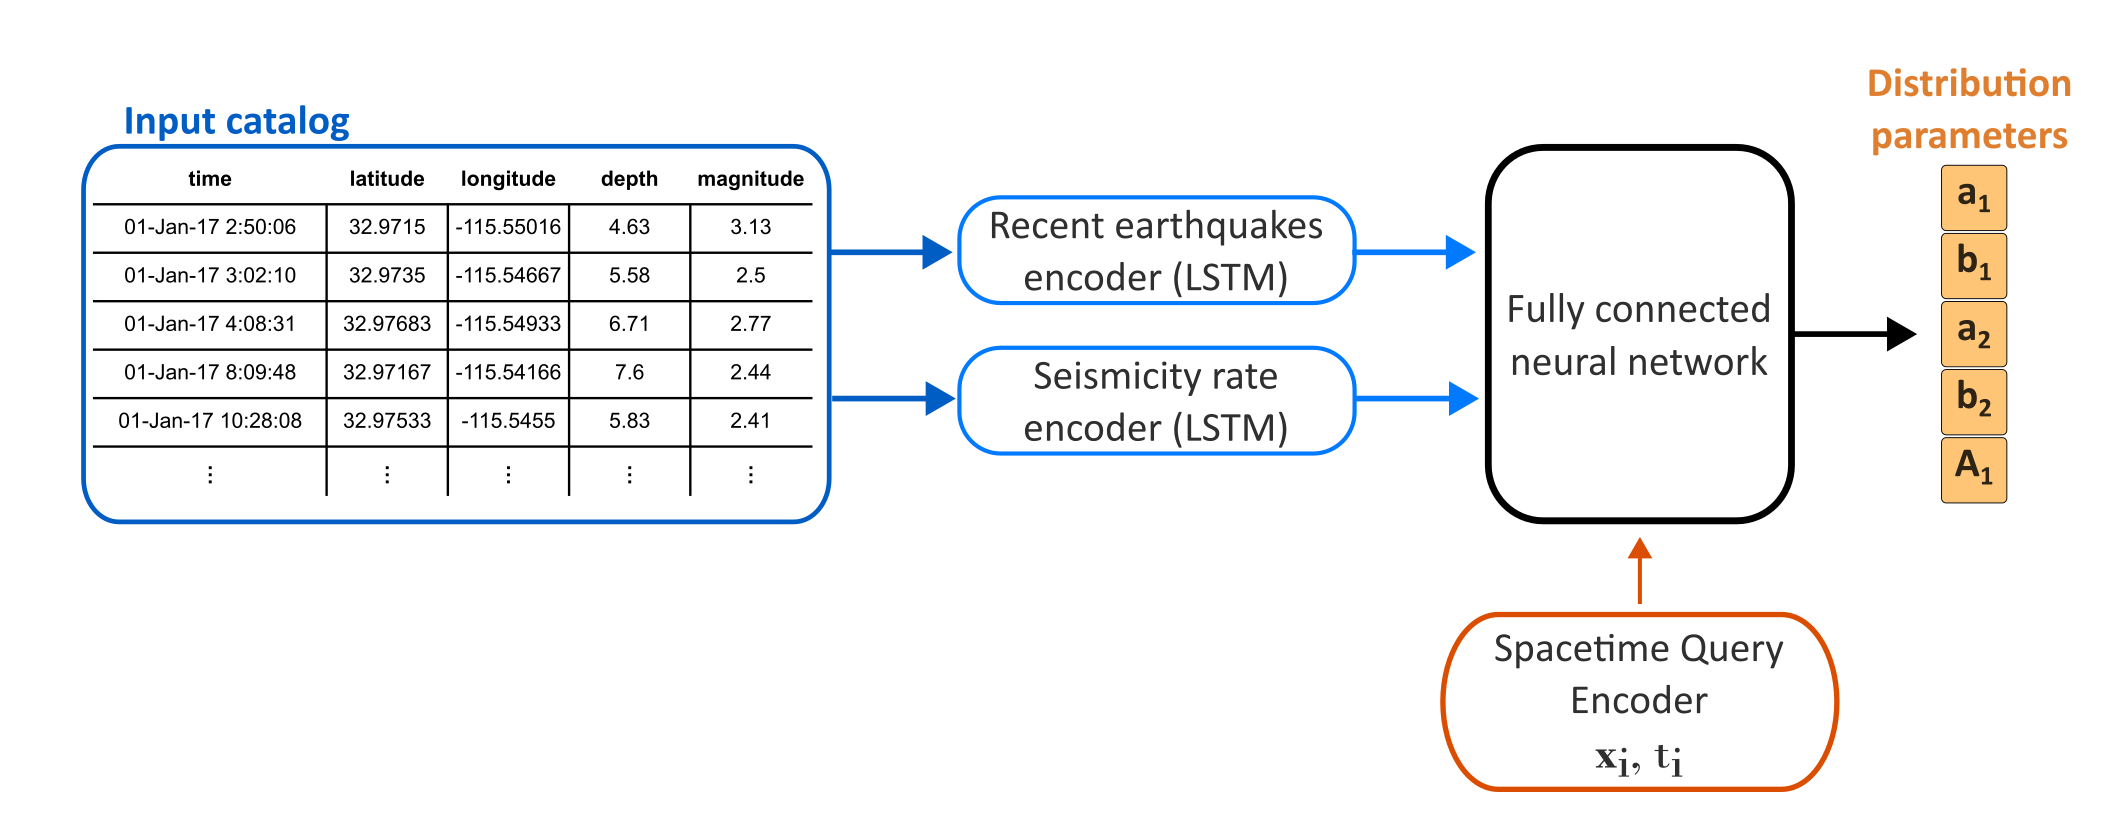
\includegraphics[width=1\textwidth]{figures/detailed_architecture.pdf}
    \caption{\textbf{MAGNET architecture.} Described in detail in the methods section.}
    \label{fig:architecture}
\end{figure}

\newpage
\begin{figure}[h!]
	\centering
        \includegraphics[width=1\textwidth]{figures/info_gain_scatter_NZ_and_Japan.png}
	\caption{
            \textbf{Information gain of MAGNET over the benchmark, New Zealand and Japan data sets.} Scattered dots indicate magnitude at event index, colored by the information gain per event. \textbf{a} Entire test set of New Zealand and a selected time span (\textbf{b}) focusing on the 2016 Te Araroa earthquake and the 2016 Kaikōura earthquake. \textbf{c} The entire Japan data set and a focused time span \textbf{d} of the 2011 Tōhoku earthquake and some of its aftershocks. Low magnitude data points in a, c and d are subsampled to ease on image rendering.
         }
\label{fig:nz_japan_info_gain}
\end{figure}

\newpage
\begin{figure}[h!]
    \centering
        \includegraphics[width=1\textwidth]{figures/temporal_incompleteness.png}
    \caption{
    \textbf{Temporal Incompleteness for test sets of all regions examined.} Calculated temporal incompleteness for test sets is presented in red, superimposed over the events above (black) and below (grey) the completeness magnitude of the train set, $m_c^{(train)}$. Events are plotted by the index of their appearance in the test set. Events of low magnitude, $m_c^{(train)}$ (grey), that are not included in the evaluation, are plotted at their interpolated location along the horizontal axis. Data for Japan (c) is displayed only near the 2011 Tōhoku earthquake to reduce data density and enhance clarity of the figure. Low magnitude data points in b and c are subsampled to ease on image rendering.
    }
    \label{fig:temp_incompleteness}
\end{figure}

\newpage
\begin{figure}[h!]
    \centering
    \includegraphics[width=1\textwidth]{figures/raw_results_em.pdf}
    \caption{
        \textbf{MAGNET’s output for Japan and New Zealand data sets}. \textbf{a} (\textbf{c}), PDFs produced by MAGNET for 100 randomly sampled events from the test set of the New Zealand (Japan) data set, with the train set’s Gutenberg-Richter distribution superimposed (dashed black line). The true magnitude label, i.e. the true magntude of the event in query, is indicated by the color, interpreted by the colorbar in a. \textbf{b} (\textbf{d}), Marginal magnitude distribution, i.e. stationary p(m), for the New Zealand (Japan) data set. Histograms of the train and test sets are presented in orange and blue respectively.
    }
    \label{fig:model_output_em}
\end{figure}

\newpage
\begin{figure}[h!]
    \centering
    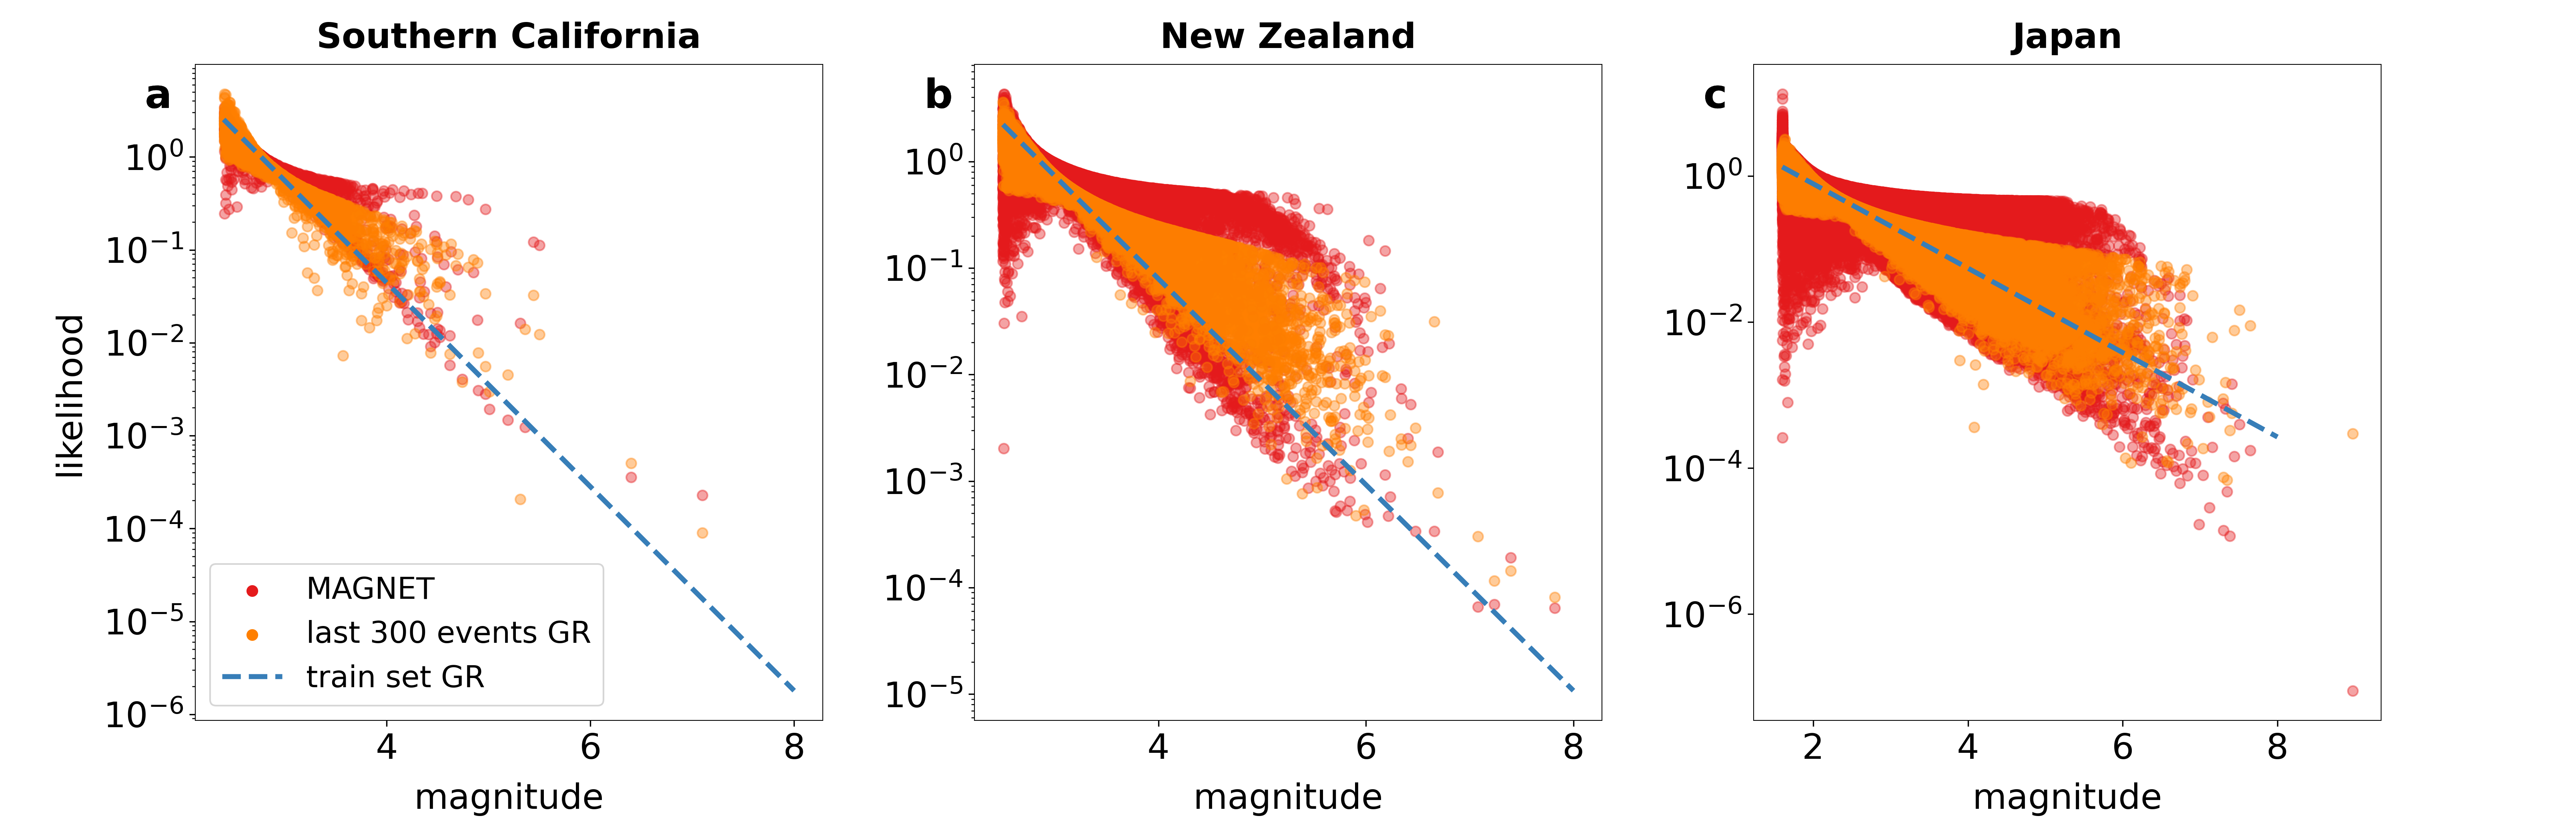
\includegraphics[width=1\textwidth]{figures/likelihood_scatter.png}
    \caption{
    \textbf{Log-likelihood of the true magnitude, $\ell_i$}. The likelihood for the true magnitude label of the test set for each data set, $\ell_i=\log\left(p_{\textbf{x}_i, t_i}(m_i)\right)$, as defined in main text. $\ell_i$ values of MAGNET and the last 300 events benchmark are shown in red and orange respectively. The blue dashed line indicates the values that the GR benchmark would obtain. Low magnitude data points in b and c are subsampled to ease on image rendering.
    }
    \label{fig:labels_likelihood}
\end{figure}


\end{document}
